\chapter{Approach Procedures}
  	\paragraph{
  		Approach Procedures are in place to ensure a safe recovery of all aircraft to their intended destination. In the 132nd we currently utilizes two types of approaches; the Straight-In Approach, and the Overhead Break.
  }

	\section{The Overhead Break}
  		\textnormal{
  			In order to expedite a speedy recovery of combat aircraft during operations, the Overhead Break (OHB) was introduced during the Second World War. This type of approach allows aircraft to keep a relatively high air speed, and to bleed of energy quickly while setting up for final, thus limiting the time it takes from crossing the threshold until safely on the ground. This is the standard approach used by the 765th. \\
  }
  
	\begin{figure}[!ht]
  		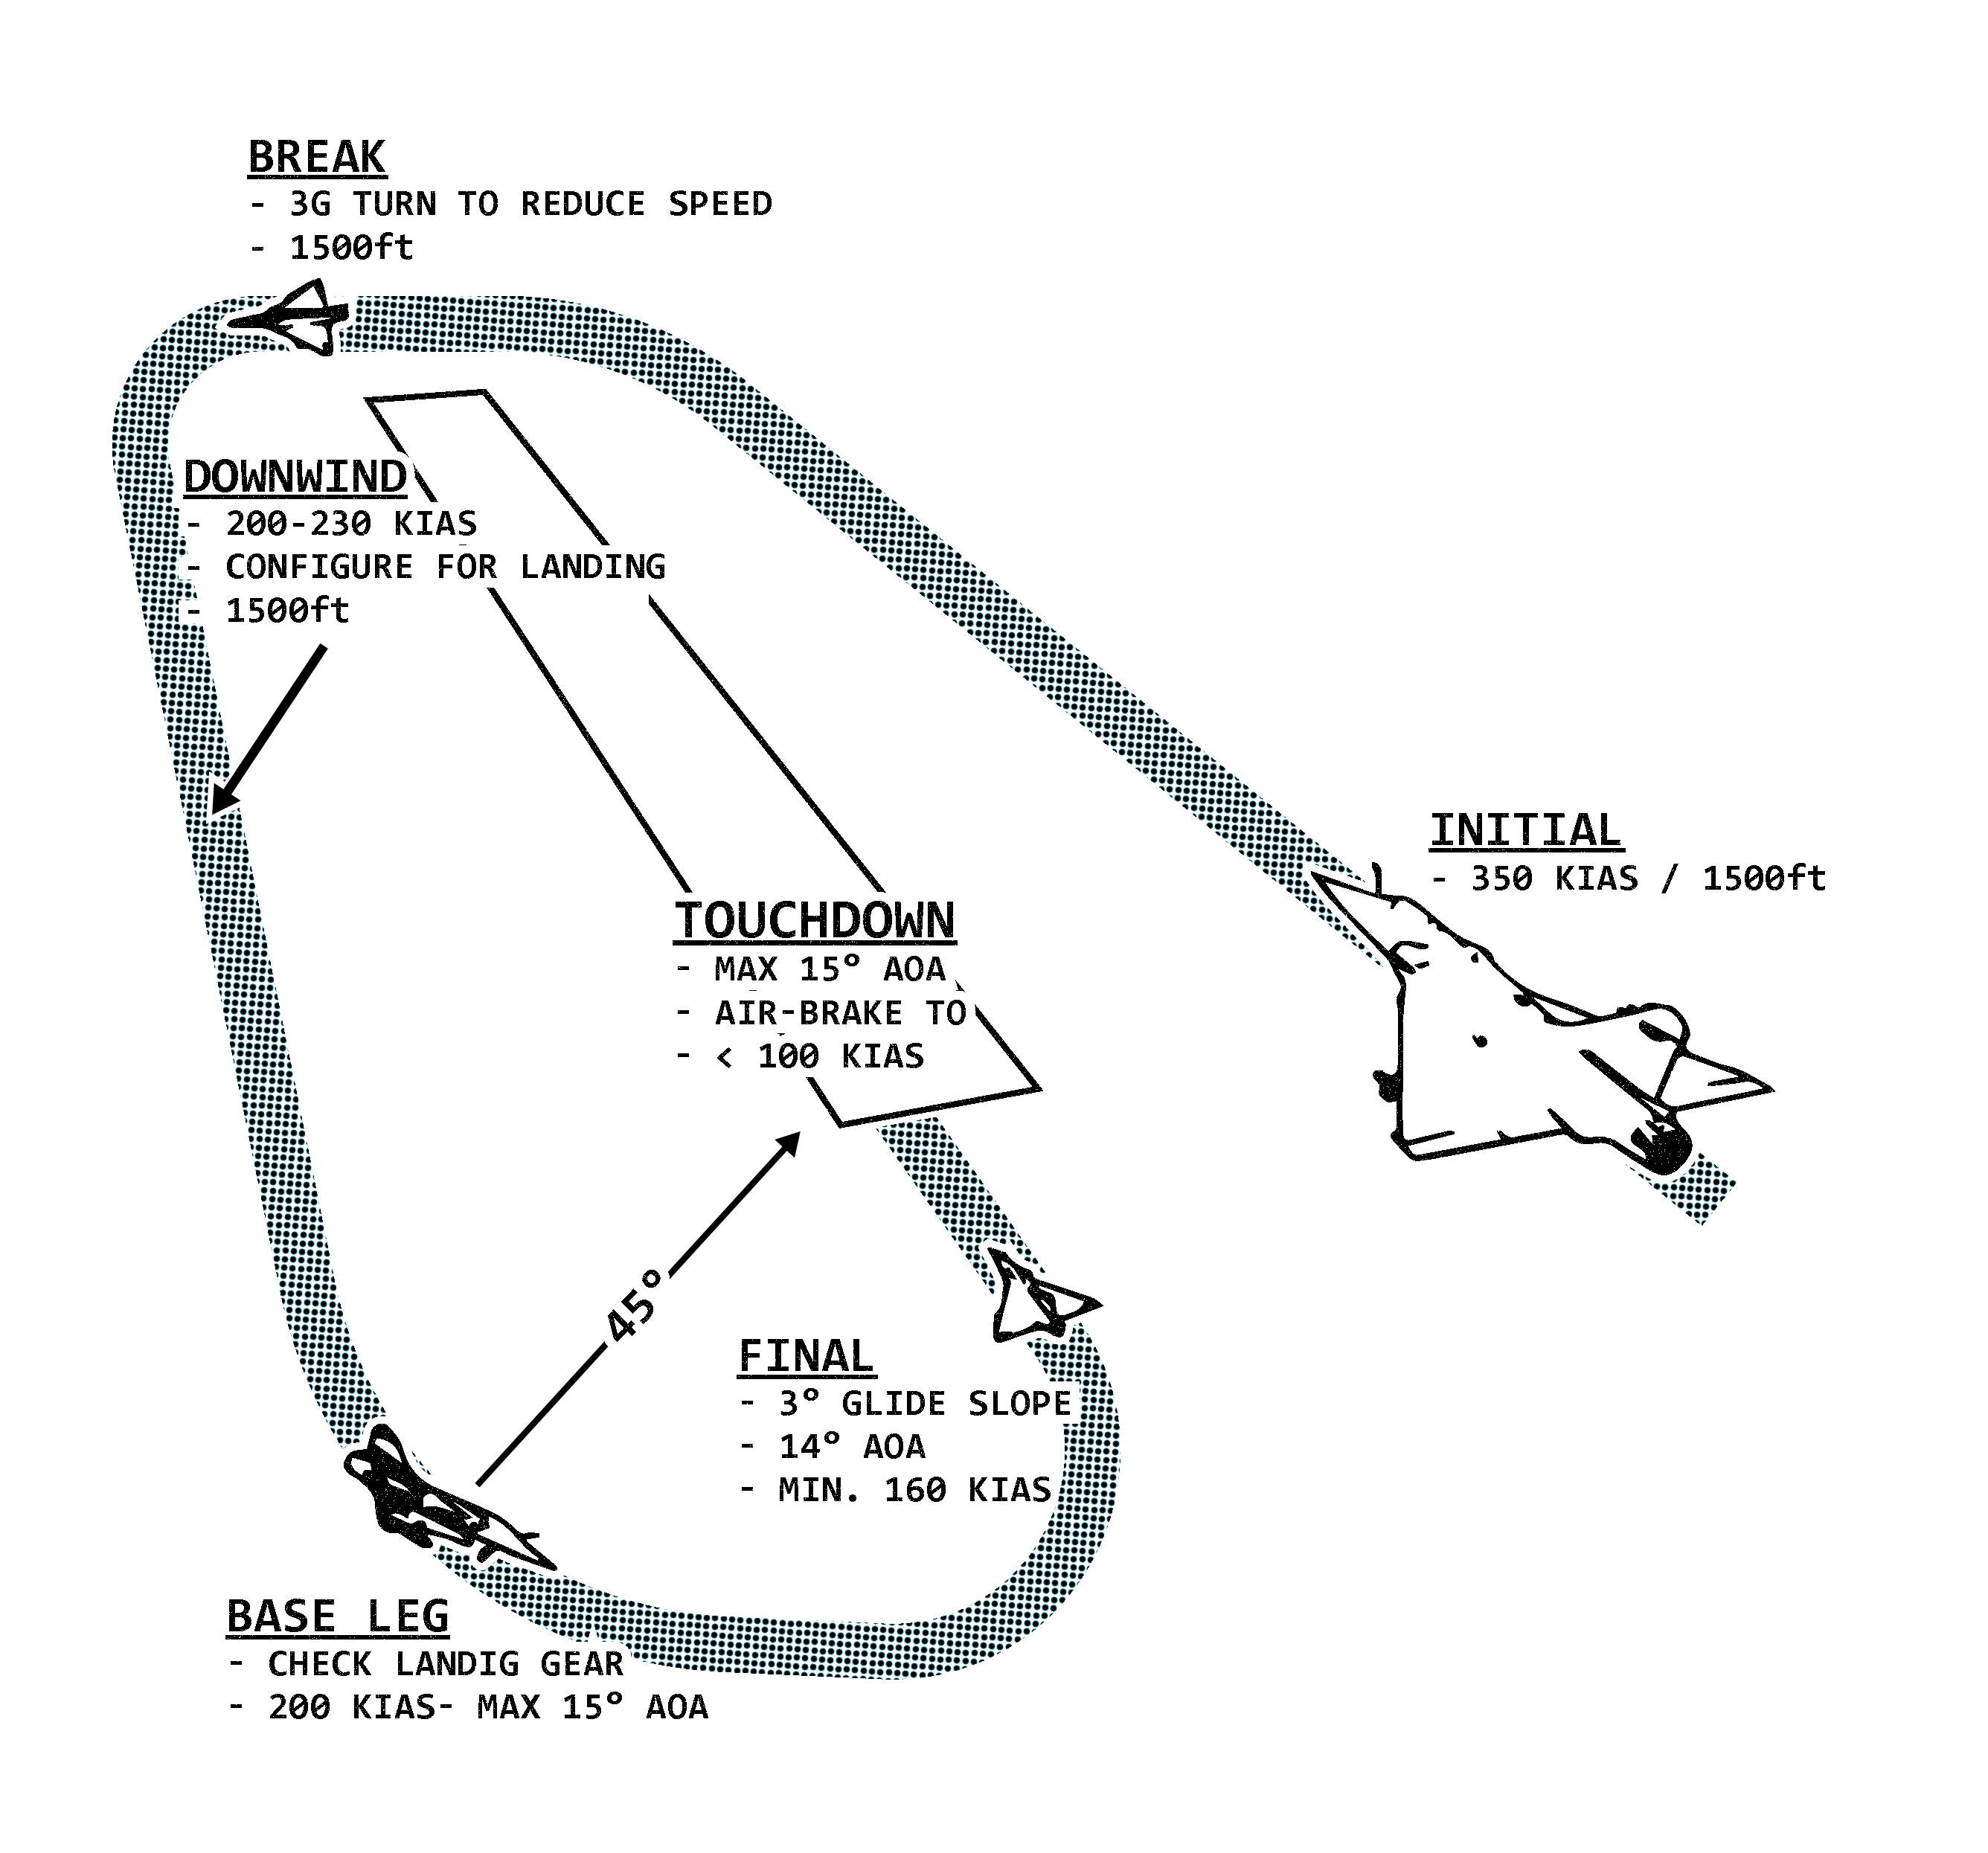
\includegraphics[scale=0.7]{ohb.png}
    		\label{ohb_fig}
    		\caption{Illustration of the Overhead Break as performed by the 765th}
  	\end{figure}